\section{Gestión del espectro radioeléctrico}

\subsection{Introducci\'on}

La Unión Internacional de Comunicaciones (ITU) \cite{ITU} ha definido el uso de cada banda de frecuencia para servicios de radio. Algunos factores como la planeación del uso de la frecuencias y características técnicas de los transmisores, receptores y antenas usadas en servicios de radio contribuyen al uso eficiente del espectro de frecuencias.
\\ \\
Las asignaciones de frecuencias en una banda para el uso de servicios de radiocomunicación espacial o terrestre son especificadas en la tabla de asignación y atribución de frecuencias de cada país.
\\ \\
Algunas naciones, realizan otros pasos.

\begin{enumerate}
\item Algunas frecuencias concuerdan con la tabla de asignación de frecuencias de la ITU y otras son definidas para evitar que algunos servicios se interfieran con los de otras naciones.
\item Un grupo de frecuencias y espacio de espectro es reservado para los últimos avances tecnológicos.
\end{enumerate}

El mundo se ha dividido en 3 regiones para propósitos de asignación de frecuencias. Los canales usados para casos especiales varían de región en región. Cada país define su propia Tabla de Asignación de Frecuencias basándose en la tabla de la ITU. \\

\begin{figure}[H]
	\centering
	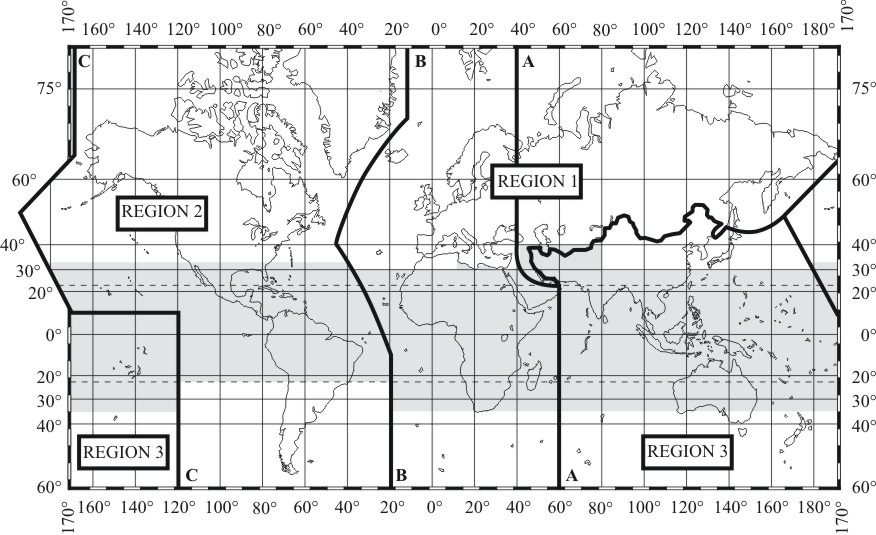
\includegraphics[width=10cm]{Capitulo2MarcoTeorico/Imagenes/ITU.png}
	\caption{División para asignación de frecuencias.}
	\caption*{Tomado del reglamento para asignaciones de frecuencia de la ITU \url{http://life.itu.ch/radioclub/image/regmap.gif}.}
	\label{fig:disitu}	
\end{figure}

\subsection{Gestión del espectro radioeléctrico en Colombia}

La gestión del espectro radioeléctrico en Colombia, es responsabilidad del estado y es un domino publico, cuya administración corresponde al Ministerio de Tecnologías de la Información y Comunicaciones (MinTIC).
\\ \\
El cuadro o tabla de asignación de frecuencias, de acuerdo a la Ley 252 de 29 de Diciembre de 1995 \cite{Ley252} y la Ley 514 de 04 de Agosto de 1999 \cite{Ley514} , corresponde al de la ITU. Este es conocido como Cuadro Nacional de Atribución de Bandas de Frecuencias.
\\ \\
Por la naturaleza dinámica de la gestión de frecuencias, el cuadro se actualiza periódicamente de acuerdo a las recomendaciones del ITU y convenios bilaterales.
\\ \\
De acuerdo a la división en regiones del mundo con respecto a la asignación del espectro, Colombia se encuentra en la Región 2.
\\ \\
En la ley 1341 del 30 de Julio de 2009 \cite{Ley1341}, se crea la Agencia Nacional del Espectro, como una unidad administrativa especial dependiente del Ministerio de Tecnologías de Información y comunicaciones, cuya función es gestionar, vigilar y controlar el espectro radioeléctrico, con excepción de los servicios de Televisión análoga y digital los cuales son administrados por la Agencia Nacional de Televisión.

\subsubsection{Cuadro nacional de atribución de frecuencias}

El cuadro nacional de atribución de frecuencias \cite{Cuadro} es un documento legal para la gestión, administración y control del espectro radioeléctrico.
\\\\
El cuadro nacional del espectro tiene las siguientes características:
\begin{itemize}
	\item Muestra todos los servicios de radiocomunicación del pais de acuerdo a la descripción de servicios de la ITU.
	\item Define la distribución del espectro radioeléctrico.
	\item Contiene referencias respecto a leyes, tratados, normas, entre otros, vinculados para el uso del espectro radioeléctrico.
\end{itemize}

Las bandas de frecuencia están definidas bajo estos conceptos:

\begin{itemize}
	\item La atribución de bandas de frecuencias a los diversos servicios de radiocomunicación comienza a partir de 9 kHz.
	\item En Colombia, la atribución nacional de frecuencias considera hasta 40,0 GHz.
	\item En Colombia, a partir de la frecuencia de 40,0 GHz y hasta la frecuencia de 1000 GHz, para fines de planeación, la atribución nacional de bandas de frecuencias es idéntica a la atribución internacional del Reglamento de Radiocomunicaciones de la ITU.
	\item La banda de frecuencias 275 - 1000 GHz no tiene actualmente atribución de servicios.
\end{itemize}

Las diferentes bandas se encuentran definidas bajo las recomendaciones de la ITU, el cuadro realiza un comparativo con la región 1, 2, 3 de la ITU con la asignación para Colombia.
\\\\
Existen dos tipos de bandas:
\begin{itemize}
	\item \textbf{Banda de frecuencia}: Estas son continuas y especifican qué servicios se presta en los diferentes bandas de frecuencia a lo largo del espectro.
	\item \textbf{Banda virtual o rango de frecuencia:} Son bandas de frecuencia definidas por servicios y con una canalización específica, es decir está dividida en segmentos los cuales pueden ser asignados, las bandas entre sí pueden solaparse o estar definidas por trozos como es el caso de la banda para el servicio de radiodifusión de televisión.
\end{itemize}

Las bandas y rangos de frecuencia pueden consultar entre las páginas 49 y 418 del cuadro nacional de atribución de frecuencias.

El cuadro nacional de atribución de frecuencias define qué servicios se prestan en el espectro radioeléctrico, los más grandes son:

\begin{itemize}
	\item \textbf{Servicio de radiocomunicación:} Todo servicio de comunicación entre un transmisor y un receptor.
	\item \textbf{Servicio Fijo:} Todos los servicios de comunicación entre estaciones fijas.
	\item \textbf{Servicio Móvil:} Agrupa los servicios que implica la comunicación con estaciones móviles.
	\item \textbf{Servicio de radioastronomía:} Son servicios aplicados a estudios en astronomía.
\end{itemize}

Los servicios pueden ser a título primario a los cuales el gobierno de Colombia se compromete a hacer respetar sus transmisiones y a título secundario los cuales pueden ser usados en una banda, pero el gobierno no garantiza que puedan ser interferidos por otros.

\subsection{Estudios económicos sobre el uso del espectro}

Para el problema de la gestión del espectro se han realizado varios estudios económicos \cite{SpectrumITU}, para estudiar el impacto de realizar una asignación determinada para una zona geográfica.
\\\\
Los costos que se deben asumir en la gestión se clasifican en:
\begin{itemize}
	\item \textbf{Costos directos:} Son los costos inmediatos de otorgar una licencia a un operador, entre los cuales se tienen, estudios de interferencia, equipos para transmisión, mover una parte congestionada del espectro y estudio de los sitios adecuados para ubicar estaciones.
	\item \textbf{Costos indirectos:} Son aquellos costos derivados de la administración del espectro, que incluye la vigilancia del uso del espectro y estudios de calidad de servicio.
\end{itemize}

Para efectos de trabajo de grado, se estudian algunos de los costos directos de la asignación del espectro los cuales son:
\begin{itemize}
	\item Costo de cambiar equipos por otros que usen mejor el espectro.
	\item Costo de mover una parte congestionada del espectro, los cuales implican el pago de compensaciones a los operadores, costos de cambio de estaciones e indemnizaciones por traumatismos para los usuarios finales.
\end{itemize}
Para efectos del trabajo de grado no se toman en cuenta los costos provocados por estudios de interferencias y ubicación de estaciones.
\\\\
Los costos indirectos no se estudian ya que son propios de la vigilancia del uso del espectro, lo que debe realizarse para garantizar se respete en la práctica la asignación realizada y es parte de los costos que no se pueden evitar en el proceso de la gestión del espectro.
\\\\
Una buena asignación del espectro busca minimizar los costos directos, buscando que la asignación sea lo más óptima posible, para evitar que se deba realizar movimiento de asignaciones para poder asignar más espectro en una banda determinada.

